\newcommand\irregularcircle[2]{% radius, irregularity
  \pgfextra {\pgfmathsetmacro\len{(#1)+rand*(#2)}}
  +(0:\len pt)
  \foreach \a in {10,20,...,350}{
    \pgfextra {\pgfmathsetmacro\len{(#1)+rand*(#2)}}
    -- +(\a:\len pt)
  } -- cycle
}
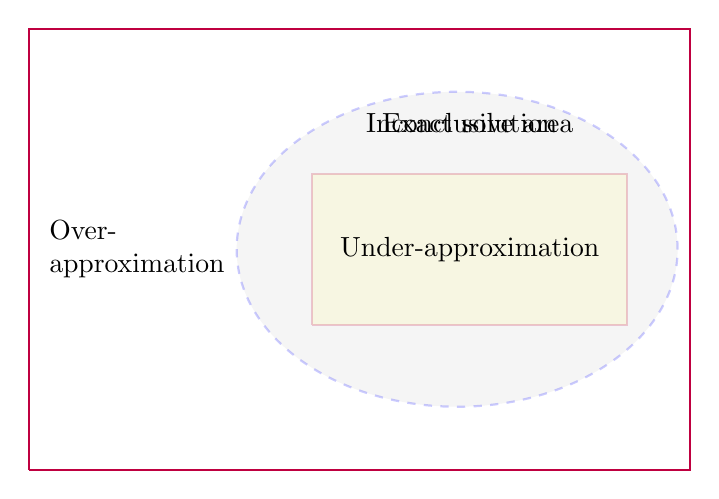
\begin{tikzpicture}[scale=0.8]
  \coordinate (c) at (-0.2,0);
  %\draw<1->[thick,blue,rounded corners=1mm,dashed,fill=gray!40,opacity=0.2] (c) \irregularcircle{3cm}{3mm};
  \draw<1->[thick,blue,rounded corners=1mm,dashed,fill=gray!40,opacity=0.2] (c) ellipse (3.5 and 2.5);
  %\draw[blue] (-1.2,-1.2) -- (1.2,-1.2) -- (1.2,1.2) -- (-1.2,1.2) -- (-1.2,-1.2);
  \draw<3->[thick,purple,fill=yellow!40,opacity=0.2] (-2.5,-1.2) -- (2.5,-1.2) -- (2.5,1.2) -- (-2.5,1.2) -- (-2.5,-1.2);
  \draw<2->[thick,purple] (-7,-3.5) -- (3.5,-3.5) -- (3.5,3.5) -- (-7,3.5) -- (-7,-3.5);
  \node<3-> (under) at (0,0) {Under-approximation};
  \node<2-> [text width=3cm] (over) at (-4.8,0) {Over-\\approximation};
  \node<1> (real) at (0,2) {Exact solution};
  \node<4> (real) at (0,2) {Inconclusive area};
\end{tikzpicture}